\subsubsection{Denormalisierung der Datenbank}
\label{ssub:denormalisierung_der_datenbank}
  Die Denormalisierung ist eine Strategie, die auf eine zuvor normalisierte Datenbank angewendet wird, um die Leistung zu erhöhen. Die Denormalisierung ist der Prozess, bei dem versucht wird, die Leseperformance einer Datenbank zu verbessern, auf Kosten der Schreibleistung, durch Hinzufügen redundanter Kopien von Daten oder durch deren Gruppierung.\parencite{sanders}
  Der große Nachteil von Denormalisierung, nämlich die Redundanz von Daten, spielt für dieses Projekt keine Rolle, da die Daten ausschließlich ausgelesen und nicht geschrieben werden. Was bleibt sind die Vorteile.\\

  Für dieses Projekt bedeutet diese Methode, eine neue Tabelle zu generieren, die den Zugriff auf die benötigten Daten einfach macht. Im Grunde handelt es sich um eine Vorberechnung. Anstatt die Tabellen bei jeder Anfrage an den Server aufwendig über viele \texttt{SQL-JOINS} zu verknüpfen, wird diese Verknüpfungen einmalig vorberechnet und in eine Tabelle gespeichert. Eine Denormalisierung  einer Tabelle ist bereits im vorherigen Abschnitt "`\nameref{ssub:aggregieren_der_shape_tabelle}"' gezeigt und führte dazu, dass die Polyline über die Abfrage einer einzigen Tabellenreihe erhalten werden kann was die Performance signifikant erhöhte. Zur besseren Verständnis soll folgende Grafik helfen:

  \begin{figure}[htbp]
    \begin{center}
      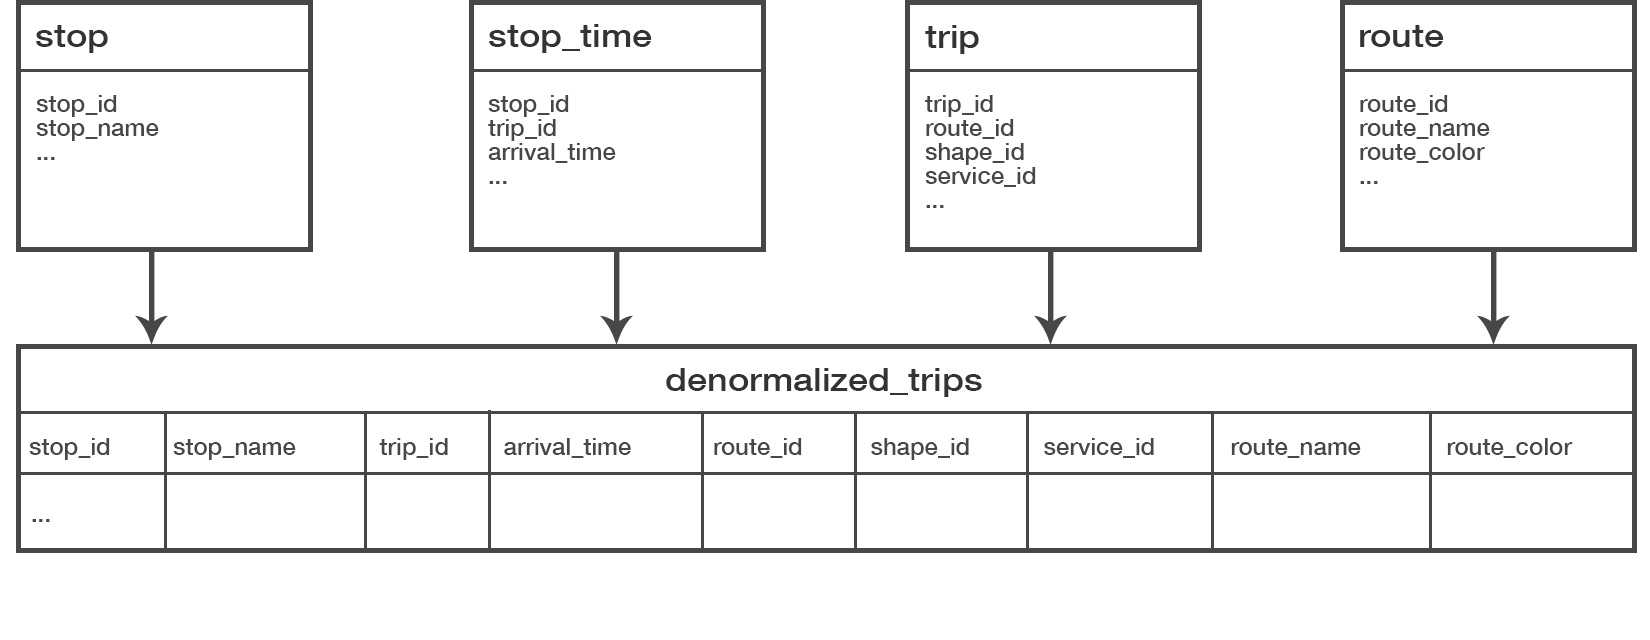
\includegraphics[width=\textwidth]{denormalizing.jpg}
      \caption{Beispiel einer Denormalisierung von Tabellen}
      \label{fig:denormalizing}
    \end{center}
  \end{figure}

  Wie in Abbildung \ref{fig:denormalizing} zu sehen ist, wird aus einer vertikalen Anordnung der einzelnen Datenfelder, eine horizontale Anordnung in einer einzigen \texttt{denormalized\_trips} Tabelle. Eine Reihe in dieser neuen Tabelle steht für genau einen Eintrag eines Trips. Anstatt also bei jeder Anfrage an den Server die verschiedenen Daten mittels \texttt{JOIN} verknüpfen zu müssen, können diese jetzt per Zugriff auf eine einzige Reihe in nur einer Tabelle erfragt werden.\\

  Dieses Prinzip, der Gruppierung von Daten in einer neuen Tabelle soll nun auch auf die anderen benötigten Tabellen angewendet werden. Die Denormalisierung erfolgt in 3 Schritten:

  \begin{enumerate}
    \item Erstellen der neuen Tabelle \texttt{denormalized\_trips}
    \item Importieren der verschiedenen Daten in diese neue Tabelle
    \item Mögliche Abfragen sind nun über diese neue Tabelle möglich.
  \end{enumerate}

  Das SQL-Statement ist abermals aufgrund seiner Länge Anhang \ref{lst:denormalized_shapes} zu entnehmen. Dies resultiert in einer Tabelle die wie folgt aussieht:

  \begin{figure}[htbp]
    \begin{center}
      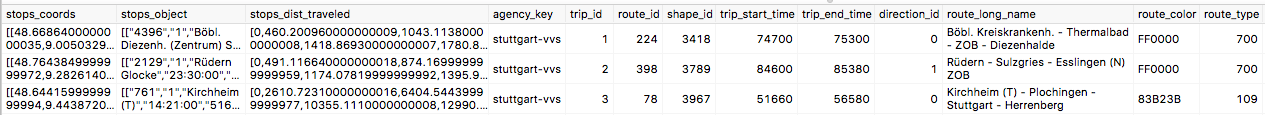
\includegraphics[width=\textwidth]{denormalized_tables.png}
      \caption{Auszug aus der \texttt{denormalized\_trips} Tabelle}
      \label{fig:denormalized_table}
    \end{center}
  \end{figure}  

  \subsubsection*{Ergebnisse}
  \label{ssub:ergebnisse}
    Für die Visualisierung ist eine Abfrage der aktiven Trips am wichtigsten.
    Folgende Tabellen werden für die Abfrage benötigt.

    \begin{figure}[htbp]
      \begin{center}
        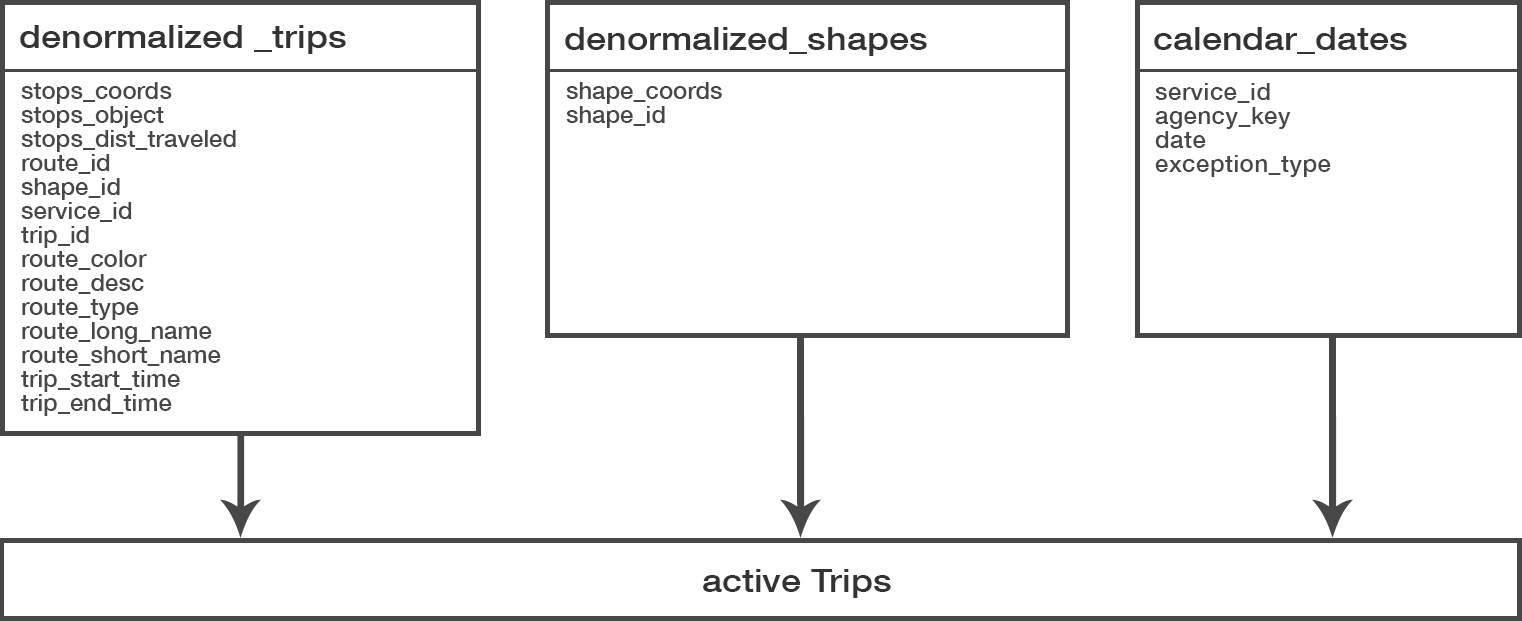
\includegraphics[width=\textwidth]{denormalizing_results.jpg}
        \caption{Benötigte Tabellen zur Abfrage von Trips}
        \label{fig:denormalizing_results}
      \end{center}
    \end{figure}

    Wie zu sehen ist, wird auf die Denormalisierte \texttt{Shape} und \texttt{Trips} Tabelle zugegriffen.

    Nachfolgend die Ergebnisse für die Abfrage von Trips in einem wachsenden Zeitrahmen. Die verwendete SQL-Abfrage befindet sich im \nameref{sec:anhang} unter Listing \ref{lst:query_trips}.

    \begin{longtable}{|>{\raggedright \arraybackslash}p{5.0cm}|>{\raggedright \arraybackslash}p{5.0cm}|>{\raggedright \arraybackslash}p{4.0cm}|}
    \caption{Evaluierung der Denormalisierung}\label{tbl:evaluierung_der_denormalisierung}\\
      \hline
        Zeitraum & Trip Anzahl & Query Zeit\\
      \hline
        9:00 bis 9:15 & 88 & 98 ms\\
        9:00 bis 10:00 & 1125 & 154 ms\\
        9:00 bis 12:00 & 3360 & 285 ms\\
        9:00 bis 15:00 & 7070 & 497 ms\\
        9:00 bis 21:00 & 14718 & 900 ms\\
      \hline
    \end{longtable}

    Die Ergebnisse Zeigen, dass die Abfragezeit der Datenbank für die aktiven Trips erheblich gesunken ist. Anfangs ist solch eine Anfrage aufgrund der endlosen Laufzeit erst gar nicht möglich gewesen.

    \pagebreak 

    \begin{figure}[htbp]
      \begin{center}
        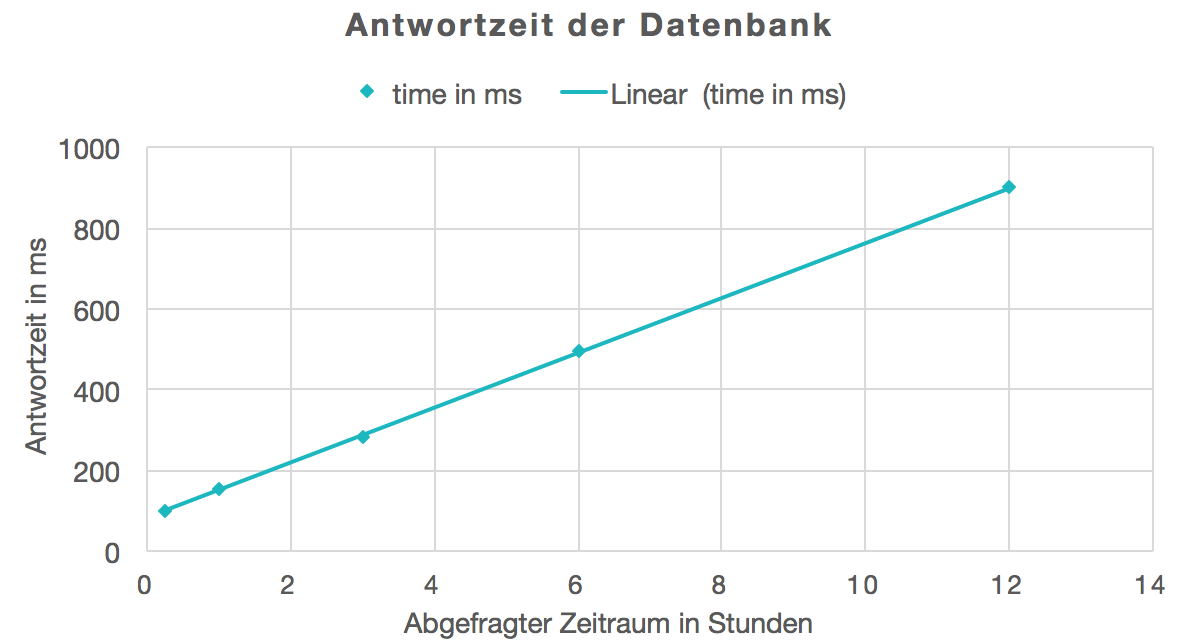
\includegraphics[width=0.65\textwidth]{query_time_chart}
        \caption{Plot der Abfragezeiten}
        \label{fig:query_time_chart}
      \end{center}
    \end{figure}
    
    Abbildung \ref{fig:query_time_chart} zeigt einen Plot der Query Zeit aus Tabelle \ref{tbl:evaluierung_der_denormalisierung} als nahezu linearen Graphen. Daraus folgt, dass die Antwortzeit der Datenbank linear mit dem abgefragten Zeitraum wächst. In der Visualisierung sind vor allem Trip Abfragen zwischen einer Minute und einer Stunde in Verwendung. Die Abfragezeit bewegt sich damit zwischen $\approx 80 -  160\; ms$.
    
  % subsubsection ergebnisse (end)

% subsubsection denormalisierung_der_datenbank (end)